\renewcommand{\FileName}{loginfl1}
\begin{frame}
  \frametitle{Influence measures and diagnostic plots}
  \begin{itemize}
	\item{\large\bfseries Leverage}: Potential impact of an individual case $\sim$ distance
	from the centroid in space of predictors
	\item{\large\bfseries Residuals}: Which observations are poorly fitted? 
	\item{\large\bfseries Influence}: Actual impact of an individual case $\sim$ leverage $\times$ residual
      \begin{itemize*}
	  \item \boldital{C}, \boldital{CBAR} -- analogs of Cook's D in OLS $\sim$ standardized change in
	  regression coefficients when $i$-th case is deleted.
		\item \boldital{DIFCHISQ}, \boldital{DIFDEV} -- $\Delta \chi^2$ when $i$-th case is deleted.
	  \end{itemize*}
  \end{itemize}
 \begin{center}
  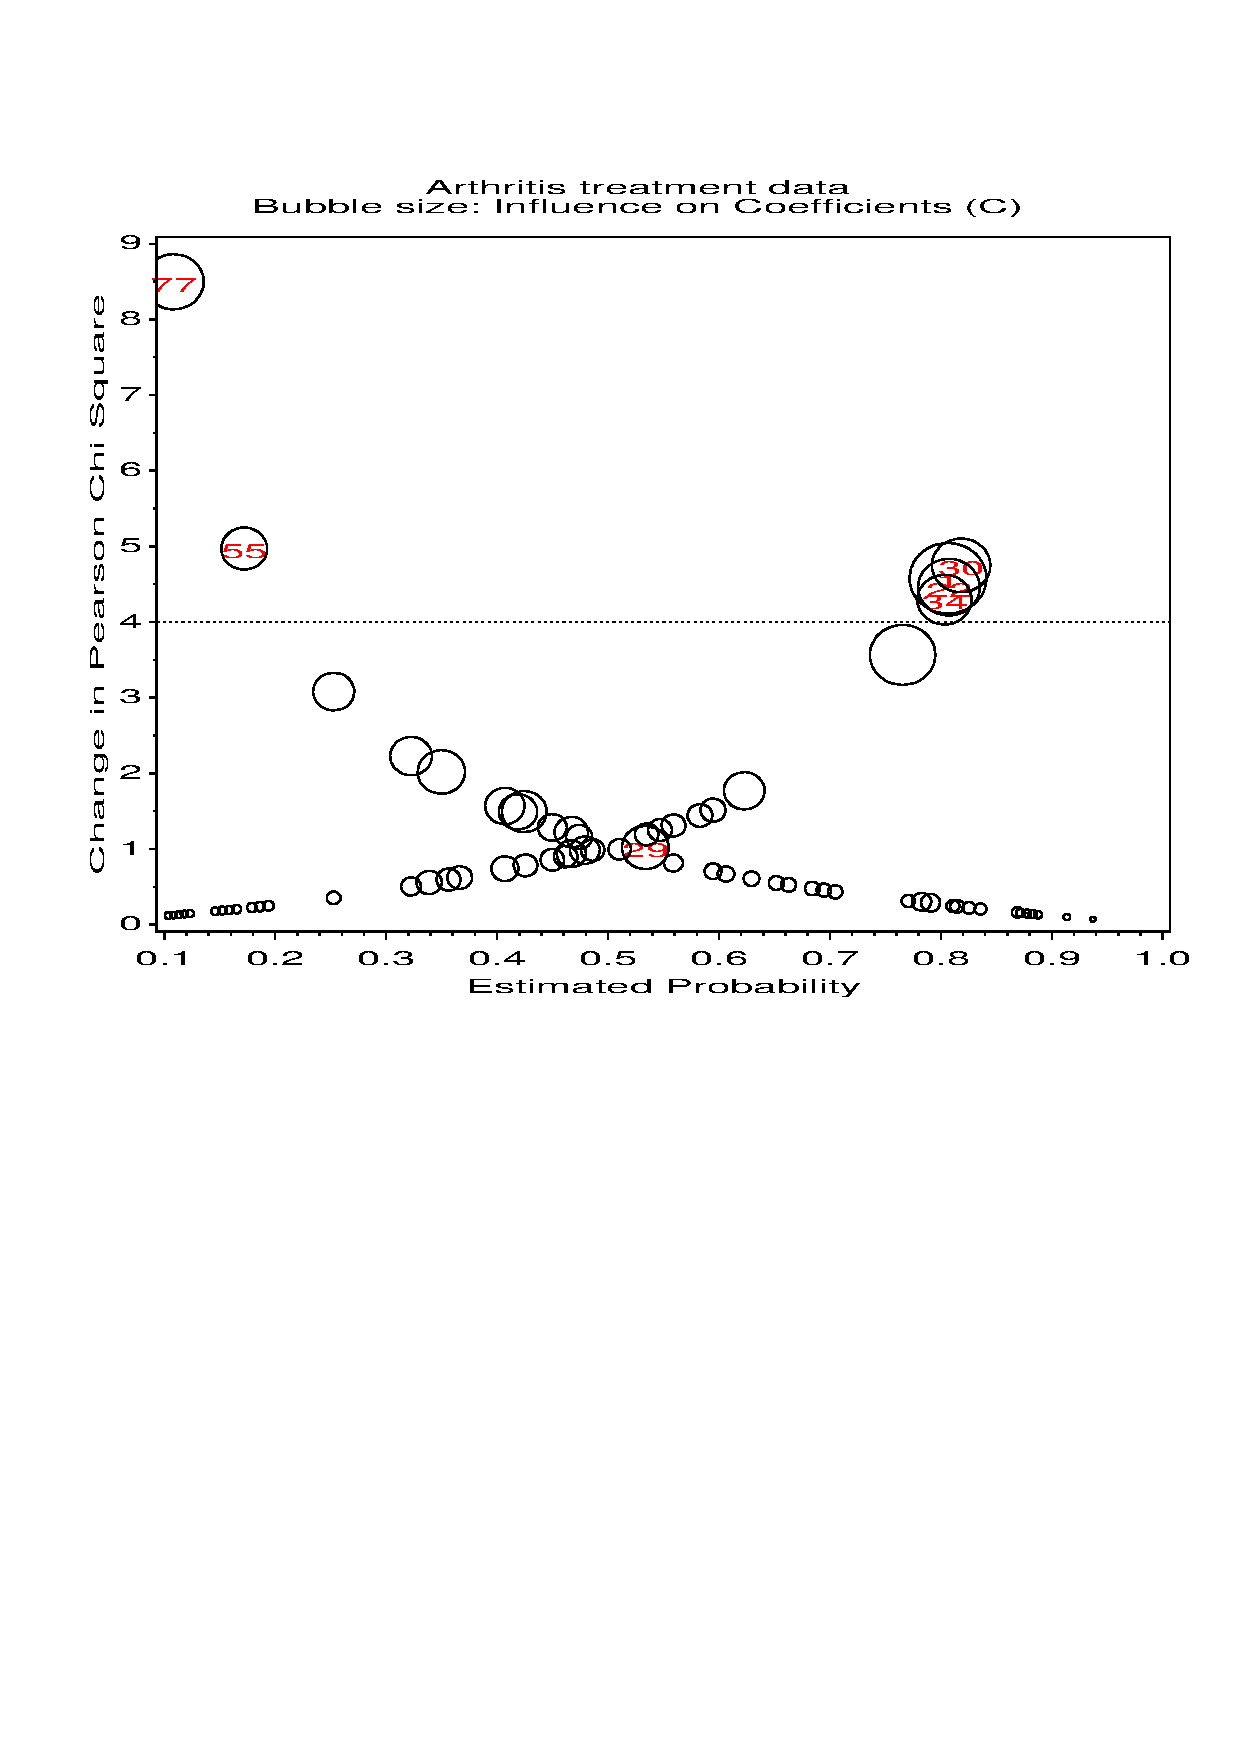
\includegraphics[width=.4\dispwidth,clip]{fig/logist1b1}
  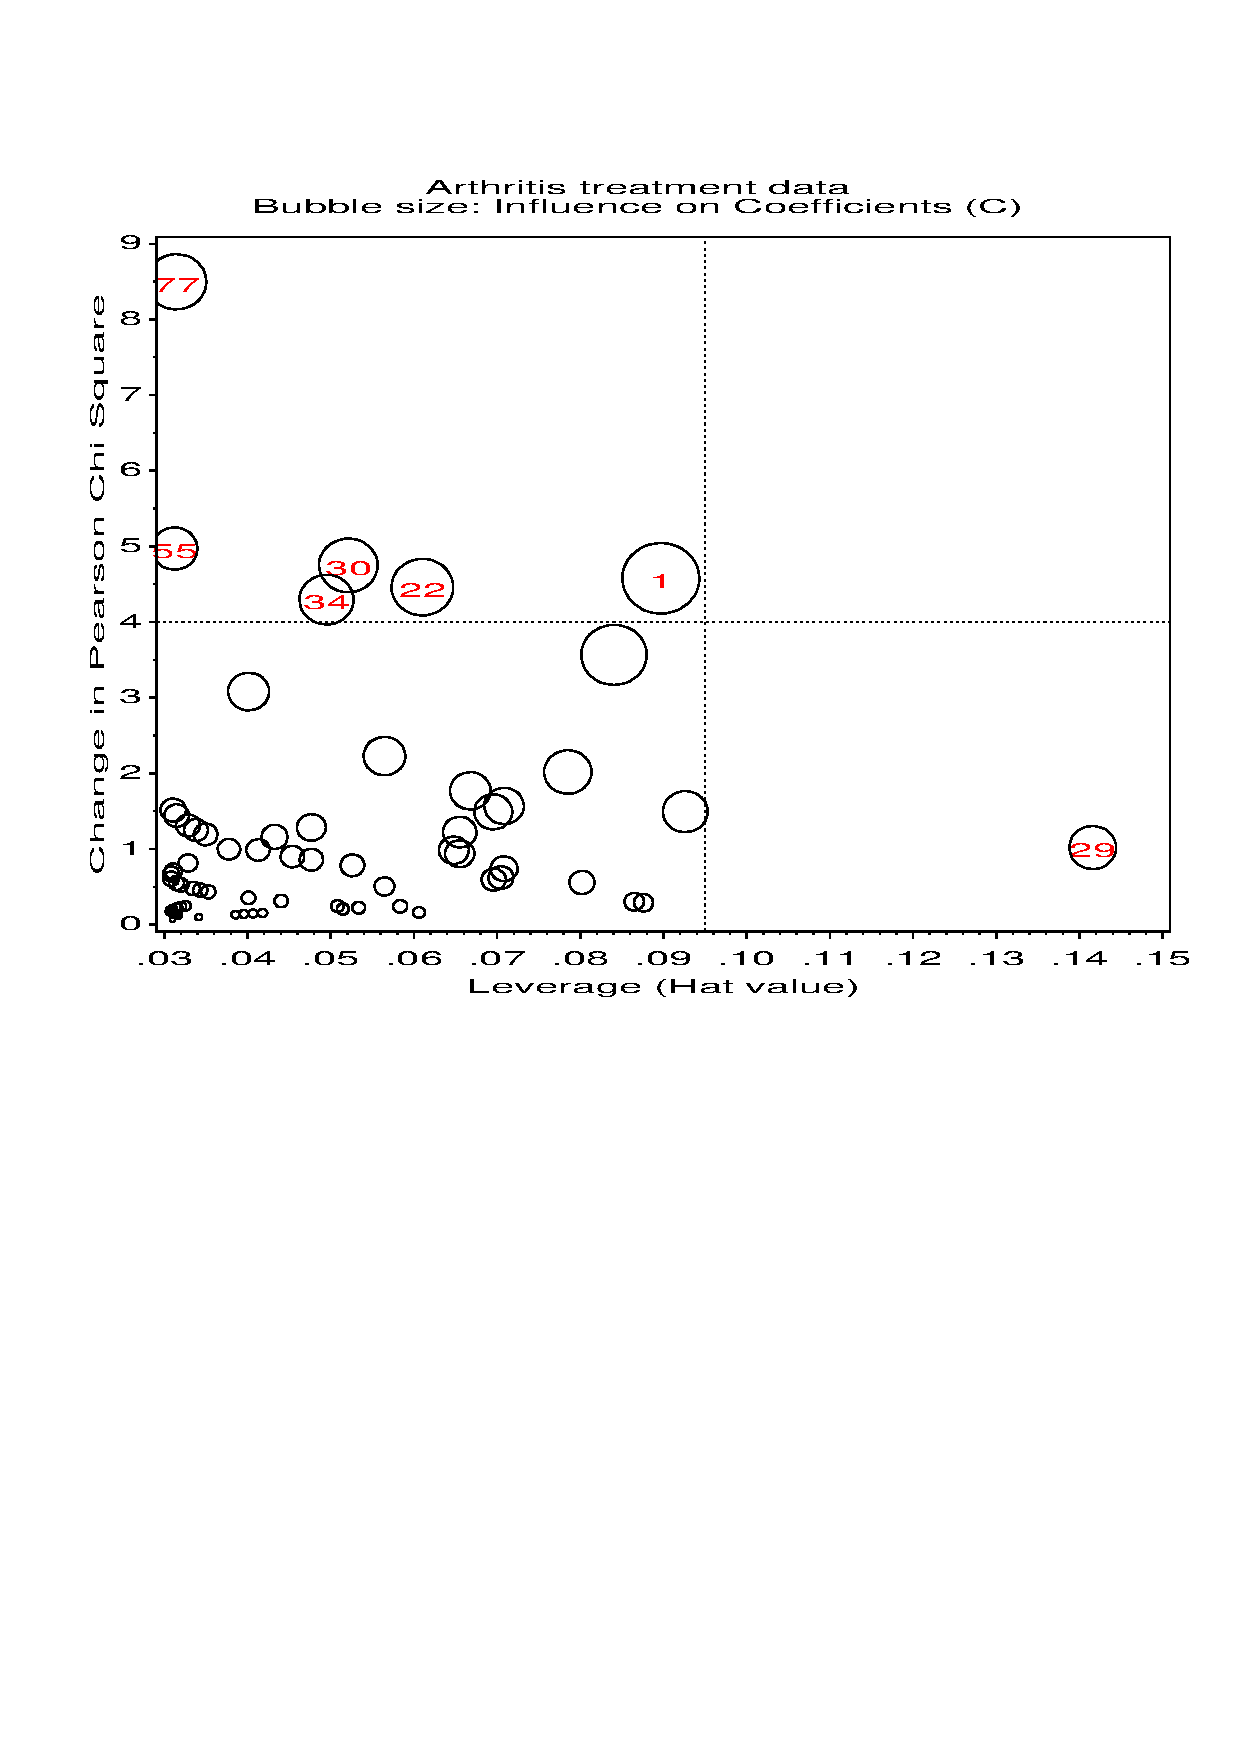
\includegraphics[width=.4\dispwidth,clip]{fig/logist1b2}
 \end{center}
\end{frame}

\begin{frame}[fragile]
  \frametitle{Influence measures and diagnostic plots}
\PROC{LOGISTIC}: printed output with the \alert{\texttt{influence}} option
\begin{Input}
proc logistic data=arthrit descending;
   model better = sex treat age / \sasemph{influence};
\end{Input}

 \begin{center}
\includegraphics[width=.85\dispwidth,clip]{fig/arthritis-influence-lst}
 \end{center}
Too much output, doesn't highlight unusual cases, ...
\end{frame}

\begin{frame}[fragile]
  \frametitle{Influence measures and diagnostic plots}
\PROC{LOGISTIC}: plotting diagnostic measures with the \alert{\texttt{plots}} option
\begin{Input}
proc logistic data=arthrit descending 
         \sasemph{plots(only label)=(leverage dpc)};
   class sex (ref=last) treat (ref=first) / param=ref;
   model  better = sex treat age ;
	run;
\end{Input}

 \begin{center}
\includegraphics[width=.49\dispwidth,clip]{fig/arthritis-influence1}
\includegraphics[width=.49\dispwidth,clip]{fig/arthritis-influence2}
 \end{center}
\end{frame}

\begin{frame}
  \frametitle{Influence measures and diagnostic plots: Influence plots}
The option \alert{\texttt{plots(label)=dpc}} gives plots of $\Delta \chi^2$ (\texttt{DIFCHISQ}, \texttt{DIFDEV}) vs. $\widehat{p}$

Points are colored according to the influence measure C.
 \begin{center}
\includegraphics[width=.85\dispwidth,clip]{fig/arthritis-influence2}
 \end{center}
The two bands of points correspond to better = \{0, 1\}
\end{frame}
